\documentclass[tikz, margin=2mm,convert={density=300,size=1920x1080,outext=.png}]{standalone}

\usepackage{xcolor}

\newcommand{\len}{7}% x direction
\newcommand{\bre}{7}% y direction
\newcommand{\hei}{4}% z direction
\newcommand{\backhei}{0.5}% for the box in behind
\newcommand{\frontcolor}{black!15!white}
\newcommand{\topcolor}{black!30!white}
\newcommand{\sidecolor}{black!45!white}

\begin{document}
    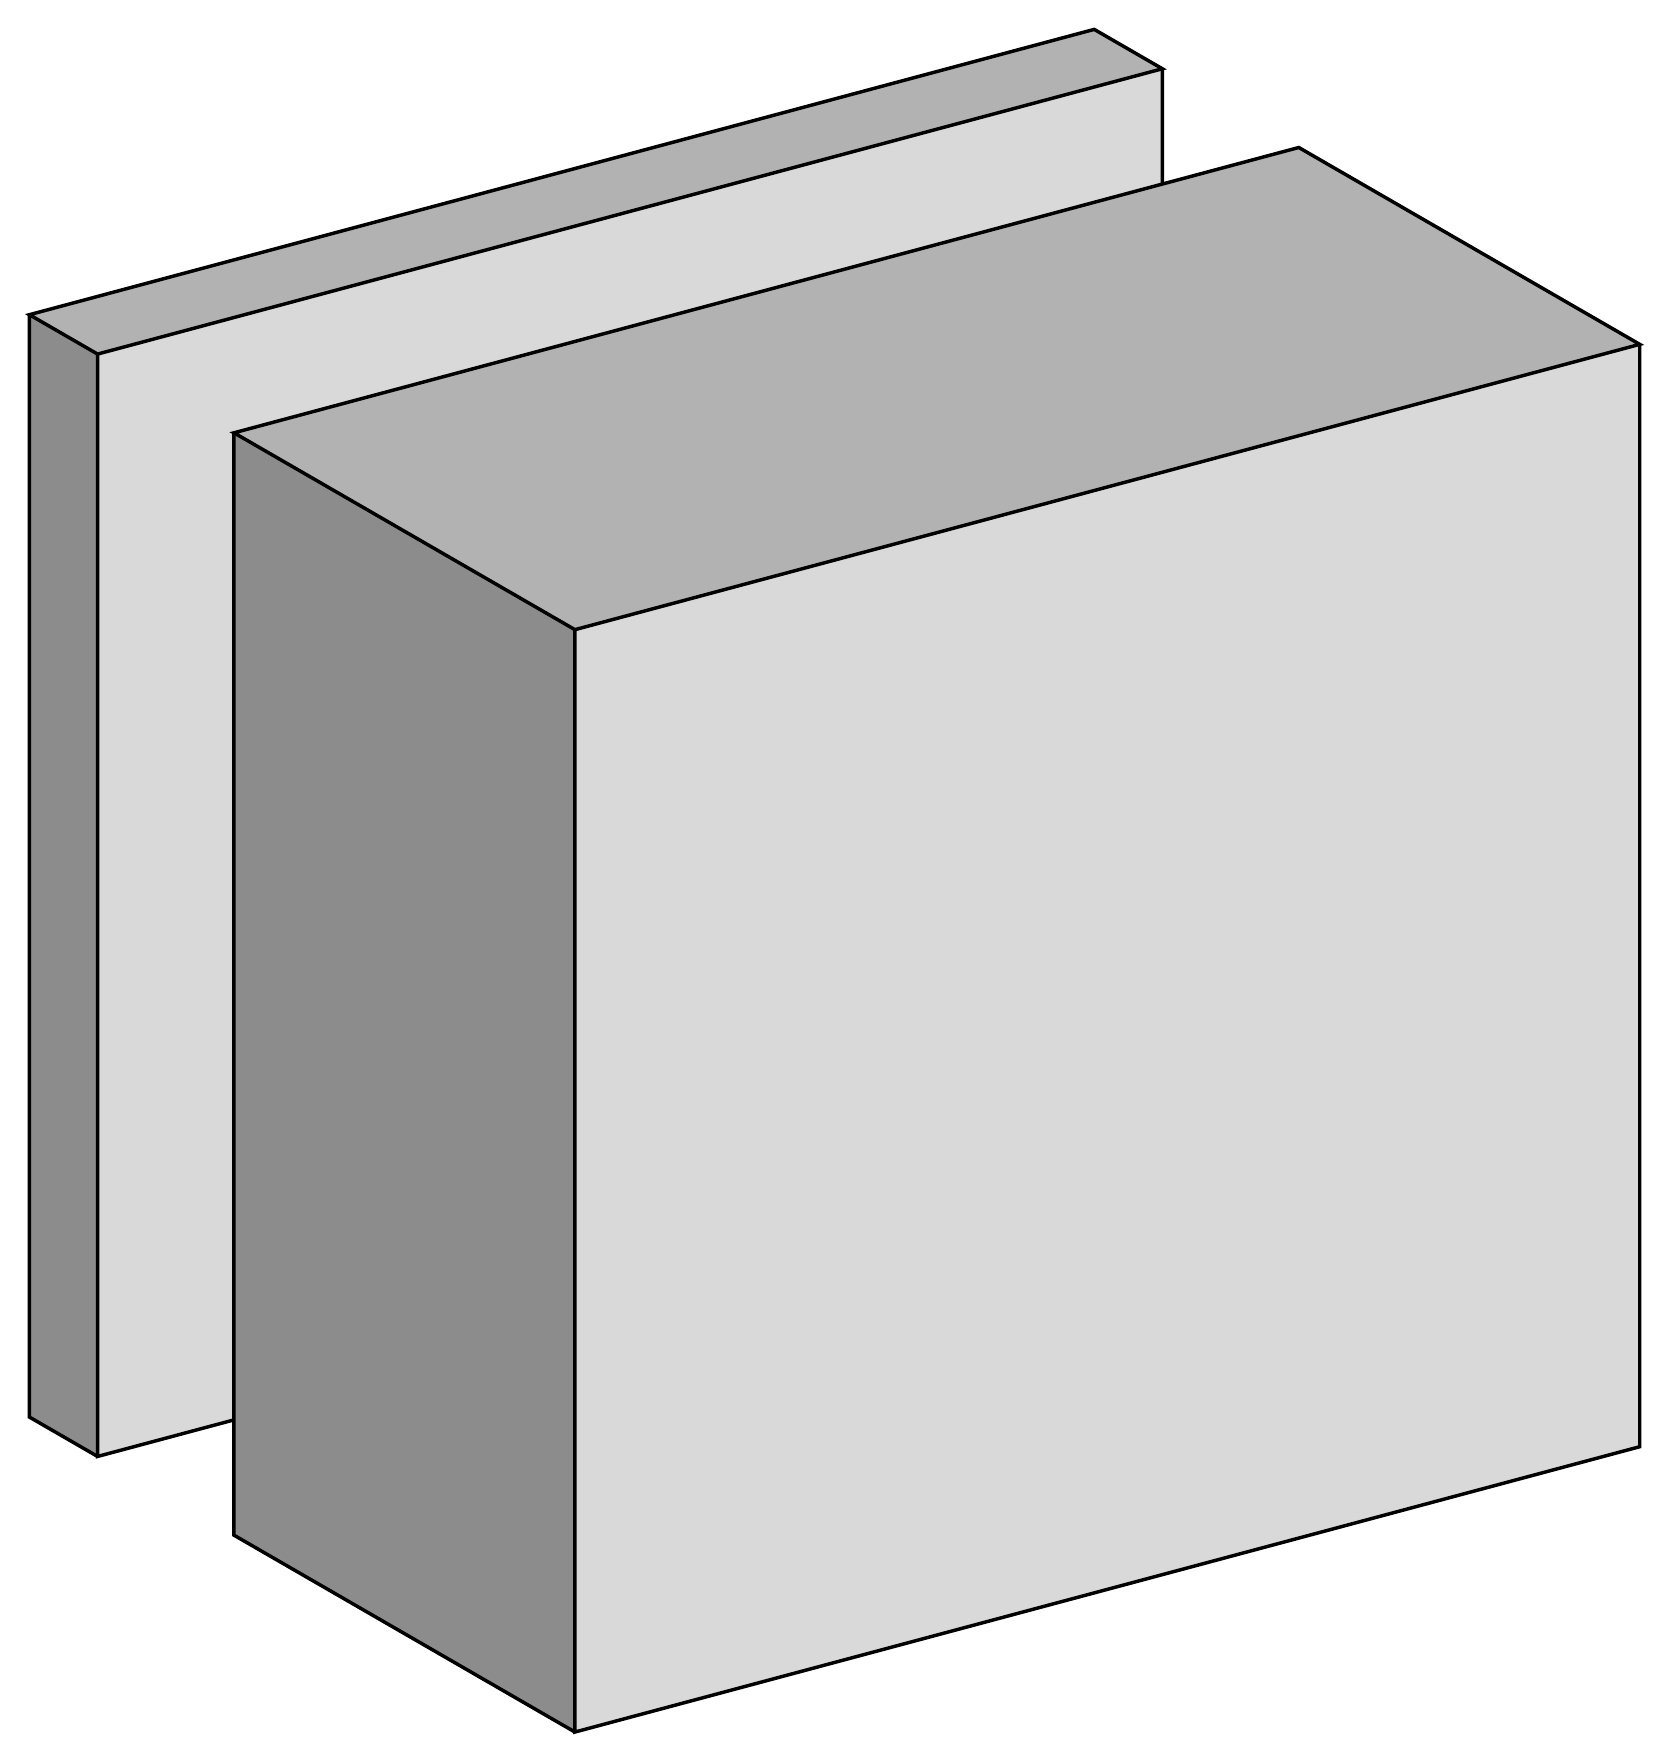
\begin{tikzpicture}[x=(15:2cm), y=(90:2cm), z=(330:2cm), >=stealth]
        \coordinate (backO) at (0, 0, 0);
        \coordinate (backA) at (\len, 0, 0);
        \coordinate (backB) at (0, \bre, 0);
        \coordinate (backC) at (\len, \bre, 0);
        \coordinate (backD) at (0, 0, \backhei);
        \coordinate (backE) at (\len, 0, \backhei);
        \coordinate (backF) at (0, \bre, \backhei);
        \coordinate (backG) at (\len, \bre, \backhei);
        
        % color
        \fill[\frontcolor] (backD) -- (backE) -- (backG) -- (backF) -- cycle;
        \fill[\topcolor] (backB) -- (backC) -- (backG) -- (backF) -- cycle;
        \fill[\sidecolor] (backO) -- (backB) -- (backF) -- (backD) -- cycle;
        
        % box edges
        \draw[line width=1.25pt] (backB) -- (backF) -- (backG) -- (backC) -- cycle;
        \draw[line width=1.25pt] (backF) -- (backD) -- (backE) -- (backG);
        \draw[line width=1.25pt] (backB) -- (backO) -- (backD);
        
        \coordinate (O) at (0, 0, \backhei+1);
        \coordinate (A) at (\len, 0, \backhei+1);
        \coordinate (B) at (0, \bre, \backhei+1);
        \coordinate (C) at (\len, \bre, \backhei+1);
        \coordinate (D) at (0, 0, \hei);
        \coordinate (E) at (\len, 0, \hei);
        \coordinate (F) at (0, \bre, \hei);
        \coordinate (G) at (\len, \bre, \hei);
        
        % color
        \fill[\frontcolor] (D) -- (E) -- (G) -- (F) -- cycle;
        \fill[\topcolor] (B) -- (C) -- (G) -- (F) -- cycle;
        \fill[\sidecolor] (O) -- (B) -- (F) -- (D) -- cycle;
        
        % box edges
        \draw[line width=1.25pt] (B) -- (F) -- (G) -- (C) -- cycle;
        \draw[line width=1.25pt] (F) -- (D) -- (E) -- (G);
        \draw[line width=1.25pt] (B) -- (O) -- (D);
    \end{tikzpicture}
\end{document}